% ----------------------------------
% 1-Preambulo.
% ----------------------------------
\documentclass[12pt,a4paper]{article}
\usepackage[spanish]{babel}
\usepackage[T1]{fontenc}
\usepackage{textcomp}
\usepackage{lmodern}
\usepackage[utf8]{inputenc}
\usepackage{graphicx}
\usepackage[procnames]{listings} 	%Para escribir códigos.
% OJO: se agregaron procnames para usarlos en Python (VER).

\usepackage[bottom]{footmisc} 	 	%Para poner las footnote al final de cada página.
\usepackage[hidelinks]{hyperref} 	%Para que el indice pueda ser linkeado.
\usepackage{amssymb}			 	%Para ecuaciones matemáticas.
\usepackage{amsmath}				%Para matrices.
\usepackage{mathtools}
\usepackage{amsfonts} 
\usepackage{verbatim}				%Para usar comentarios.
\parskip 0.1in 						%Distancia parrafos.

%Biliografías:
%\usepackage[style=authoryear]{biblatex}
%\addbibresource{bibliografias.bib}

\usepackage{float} 							%Para que no se muevan las imágenes de lugar.

\usepackage[
  separate-uncertainty = true,
  multi-part-units = repeat
]{siunitx} 									%Para el \SI del +- .

\usepackage[margin=0.984252in]{geometry} 	%Para los márgenes.
\usepackage{subcaption}
\usepackage{appendix} 						%Para los anexos.

% ----------------------------------
% 1.1-Anexos.
% ----------------------------------

%begin anexos
\makeatletter
\def\@seccntformat#1{\@ifundefined{#1@cntformat}  	%"\@seccntformat" es un comando auxiliar.
   {\csname the#1\endcsname\quad}  					%Default.
   {\csname #1@cntformat\endcsname}					%Enable individual control.
}

\let\oldappendix\appendix 							%Guarda la definicion vigente de \appendix
\renewcommand\appendix{%
    \oldappendix
    \newcommand{\section@cntformat}{\appendixname~\thesection\quad}
}
\makeatother
%\renewcommand{\appendixname}{Anexos}
%\renewcommand{\appendixtocname}{Anexos}
%\renewcommand{\appendixpagename}{Anexos}
%end anexos

% ----------------------------------
% 1.2-Para código Python. 
% ----------------------------------
\usepackage{color}
\definecolor{keywords}{RGB}{255,0,90}
\definecolor{comments}{RGB}{0,0,113}
\definecolor{red}{RGB}{160,0,0}
\definecolor{green}{RGB}{0,150,0}
 
\lstset{language=Python, 
        basicstyle=\ttfamily\small, 
        keywordstyle=\color{keywords},
        commentstyle=\color{comments},
        stringstyle=\color{red},
        showstringspaces=false,
        identifierstyle=\color{green},
        procnamekeys={def,class}}

% ----------------------------------
% 1.3-Índice. 
% ----------------------------------

\setcounter{secnumdepth}{3} 		%Para que ponga 1.1.1.1.
\setcounter{tocdepth}{4} 			%Para que añadir las secciones en el Índice.
\usepackage{chngcntr}				%Para que el número de las figuras esten acordes a la sección.
\counterwithin{figure}{section}

\author{
  Calonge, Federico Matias\\
  \text{calongefederico@gmail.com}
}

\title{
  Tesis \\
  \large Automatización de lectura de Curriculum Vitae  \\
    para selección de personal en el Sector IT}
    
%Para modificar los parrafos y para que se pueda poner subsections:
\makeatletter
\renewcommand\paragraph{\@startsection{paragraph}{4}{\z@}
            {-2.5ex\@plus -1ex \@minus -.25ex}
            {1.25ex \@plus .25ex}
            {\normalfont\normalsize\bfseries}}
\makeatother
\setcounter{secnumdepth}{4} 	%How many sectioning levels to assign numbers to.
\setcounter{tocdepth}{4}    	%How many sectioning levels to show in ToC.
% ----------------------------------
% 2-Documento
% ----------------------------------

\begin{document}

\begin{figure}
  \centering
  
\includegraphics[width=0.2\textwidth]{images/undav-logo.png} 	%Incluyendo logo de la Undav.
  \label{fig:undav-logo}
\end{figure}
\maketitle       		%Para generar el título definido arriba.

\cleardoublepage    %Nueva página

\begin{center}
    \Large
    \vspace{0.9cm}
    \textbf{Resumen}
    
\end{center}

En la Tesis de Ingeniería en Informática que se presenta, se diseña un \textit{sistema de lectura automática de Curriculum Vitae} accesible vía Web. La finalidad del mismo es ayudar al reclutador laboral a elegir a los mejores candidatos para los puestos laborales de IT que tenga disponible. Esta elección se realiza mediante el uso de algoritmos de Machine Learning y basándose, principalmente, en una medición de similitud entre textos: Curriculum Vitae de los candidatos por un lado, y descripciones de los puestos laborales de IT por el otro.
El sistema esta desarrollado utilizando el lenguaje de programación Python, permitiendo verificar la teoría desarrollada.

\begin{center}
    \Large
    \vspace{0.9cm}
    \textbf{Abstract}
\end{center}

This Computer Engineering Thesis introduces an \textit{automatic Curriculum Vitae reading system} accesible via the Web. The purpose of it is to help the job recruiter to choose the best candidates for the available IT job positions. This choice is made through the use of Machine Learning algorithms and based mainly on a measurement of similarity between texts: Curriculum Vitae of the candidates on the one hand, and IT job descriptions on the other hand.
The system is developed using the Python programming language allowing to verify the developed theory.

\cleardoublepage    %Nueva página

\tableofcontents 	%Para insertar el índice general.

\cleardoublepage    %Nueva página

\section{Introducción.}
El proceso de \textbf{selección de personal} se ha vuelto crucial para el manejo de recursos humanos en el mundo laboral moderno. Con la transformación digital de las empresas y del mercado laboral en general, identificar los perfiles más acordes a las necesidades de la empresa se convirtió en uno de los retos más ambiciosos de Recursos Humanos, en especial cuando hablamos del \textbf{Sector IT}, donde año a año se van generando nuevos puestos de trabajo. 

En estos últimos años se implementaron una gran cantidad de \textbf{herramientas de Software que permiten automatizar y gestionar información de los candidatos de una manera mucho más intuitiva e inteligente}. Gracias a la ayuda de este tipo de sistemas, el reclutador consigue a los candidatos más cualificados para cada puesto.

El tema de este Proyecto de Tesis será desarrollar un \textit{sistema de lectura automática de Curriculum Vitae} accesible vía Web. La finalidad del mismo es ayudar al reclutador laboral a elegir a los mejores candidatos para los puestos laborales de IT que tenga disponible. Esta elección se realiza mediante el uso de algoritmos de Machine Learning y basándose, principalmente, en una medición de similitud entre textos: Curriculum Vitae de los candidatos por un lado, y descripciones de los puestos laborales de IT por el otro.

La medición de similitudes de documentos es uno de los problemas más cruciales del \textbf{Procesamiento del Lenguaje Natural (NLP)}. Encontrar similitudes entre documentos se utiliza en varios dominios, tales como recomendación de películas, libros o artículos similares, identificación de documentos plagiados o documentos legales, etc. 

Para que las máquinas puedan descubrir esta similitud entre documentos, se necesita definir una forma de medir matemáticamente la similitud, la cual debe ser comparable para que la máquina pueda identificar qué documentos son más similares (o menos). Previamente a esto necesitamos representar el texto de los documentos en una forma cuantificable (que suele ser en forma vectorial), de modo que podamos realizar cálculos de similitud sobre él.

Por lo tanto, los pasos necesarios para que las máquinas puedan medir la similitud entre documentos son:
\begin{enumerate}
\item Convertir un documento en un objeto matemático (vector).
\item Definir y emplear una medida de similitud.
\end{enumerate}

Para el primer paso se utilizarán los algoritmos de vectorización \textbf{TF-IDF} y \textbf{Word Embeddings}; y para el segundo paso se emplearán las técnicas \textbf{Cosine Similarity} y \textbf{Word Mover's Distance -WMD-}.

Una vez obtenidos estos valores de .... lo que se hará es .... (KNN y K-MEANS).

\cleardoublepage    %Nueva página

\subsection{Objetivos del Proyecto.}

\subsubsection{Objetivo general.}

El objetivo de este Proyecto de Tesis es lograr un desarrollo, tanto teórico como práctico, de un \textit{sistema de lectura automática de Curriculum Vitae} accesible vía Web. La finalidad del mismo es ayudar al reclutador laboral a elegir a los mejores candidatos para los puestos laborales de IT que tenga disponible. Esta elección se realiza mediante el uso de algoritmos de Machine Learning y basándose, principalmente, en una medición de similitud entre textos:  
\begin{itemize}
\item los Curriculum Vitae de los candidatos por un lado, 
\item y descripciones de los puestos laborales de IT por el otro.
\end{itemize} 

\subsubsection{Objetivos específicos.}
Los objetivos específicos de este Proyecto de Tesis son:
\begin{itemize}
\item Describir el estado del arte actual de los Sistemas de lectura y análisis de Curriculum Vitae en Recruiting. 
\item Implementar un Sistema de lectura automática de Curriculum Vitae basado en la comparación entre textos, para finalmente obtener una visualización de los mejores candidatos para un puesto laboral de IT determinado.  
\item Aprender los conceptos y técnicas principales utilizadas dentro del procesamiento de lenguaje natural (NLP) aplicando técnicas de preprocesamiento y limpieza de textos.
\item Implementar diferentes técnicas para medir similitudes entre los textos (Cosine Similarity y  Word Mover's Distance -WMD-) y diferentes algoritmos de vectorización (TF-IDF y Word Embeddings), analizando su funcionamiento tanto teórica como matemáticamente, ventajas y desventajas.
\item Evaluar los resultados de cada técnica y algoritmo e implementar la mejor solución en el Sistema.
\item Evaluar los Frameworks disponibles para tener una UI accesible vía web e integrar el mismo al Sistema.
\item Almacenar datos de Candidatos, Reclutadores y puestos laborales en una base de datos; contando con un sistema de login y registración para los mismos.
\end{itemize} 

\cleardoublepage    %Nueva página

\subsection{Alcance del Proyecto.}
El alcance de esta Tesis de Grado de Ingeniería incluye el desarrollo de conceptos de análisis de datos, procesamiento de lenguaje natural, técnicas de preprocesamiento y limpieza de los datos, algoritmos de vectorización y técnicas para medir la similitud entre textos, integración con frameworks, visualización de datos, y gestión de Base de Datos, de acuerdo a lo enunciado en los objetivos específicos.

\subsection{Organización.}
Este Proyecto de Tesis consiste en tres grandes secciones:
\begin{enumerate}

\item Análisis e investigación inicial. Esta sección abarca principalmente la parte teórica del trabajo, haciendo hincapié en el análisis e investigación de:
\begin{itemize}
	\item El estado del arte (actual y pasado) de los sistemas de lectura y análisis de Curriculum Vitae.
	\item Técnicas usadas para el procesamiento del lenguaje natural (NLP).
	\item Técnicas para medir similitudes entre textos: Cosine Similarity y WMD.
	\item Algoritmos de Vectorización: .... y .... .
	\item Algoritmos de Machine Learning de aprendizaje supervisado (KNN) y no supervisado (K-means).
\end{itemize} 

\item Investigación e implementación del algoritmo core del sistema. Esta sección hace referencia a la aplicación práctica dentro del marco teórico desarrollado en la primera sección, la cual abarca:
\begin{itemize}
	\item Obtención de sets de datos: curriculums vitaes y descripciones laborales. 
	\item Preprocesamiento de los textos.
	\item Implementación del algoritmo CORE: utilizando las técnicas para medir similitudes entre textos (... y ....), algoritmos de vectorización (... y ...) y los algoritmos de ... (KNN y K-means).
	\item Pruebas entre distintas técnicas y librerías disponibles. 
	\item Análisis y primeras visualizaciones de los resultados.
\end{itemize} 
	
\item Investigación e implementación de la parte funcional del sistema. Esta última sección abarca lo que es la interfaz de usuario y su integración a un sistema web capaz de manejar las actividades entre los Candidatos y Reclutadores dentro del sistema. Los items principales son:
\begin{itemize}
	\item Definición de usuarios y roles.
	\item Integración de frameworks y bases de datos.  
	\item Modelado, filtrado y visualización de los datos.
\end{itemize} 

\end{enumerate}

\colorbox{red}{VER si poner de primero hacer análisis en Jupyter notebooks -sección 2-}\\
\colorbox{red}{y despues la parte web en django integrando estos jupyters -sección 3-}\\

\cleardoublepage    %Nueva página

\section{Reclutamiento laboral en IT.}
En este capítulo se va a realizar una introducción a la historia del Reclutamiento laboral, especialmente en el sector de IT, sus etapas y problemáticas.
Luego se realizará un análisis del Estado de Arte actual de los Sistemas de lectura y análisis de CV actuales.

\subsection{Introducción.}
\colorbox{red}{FALTA}

El proceso de contratación fue evolucionando a lo largo del tiempo. En el modelo de contratación de primera generación, las empresas anunciaban sus vacantes de puestos laborales en diarios, revistas, radio y televisión. Los candidatos enviaban sus currículums por correo postal y sus currículums se clasificaban manualmente. Una vez preseleccionados los candidatos, el equipo de contratación llamaba a los mismos para realizar rondas de entrevistas. Este fue un procedimiento que llevó mucho tiempo.
Luego de esto pasamos a la segunda generación. En esta época las empresas comenzaron a crecer y también lo hicieron las necesidades de contratación. Las empresas empezaron a subcontratar su proceso de contratación naciendo de esta manera las consultoras o agencias de contratación. Estas consultoras requerían que los solicitantes cargaran sus currículums en sus sitios web en formatos particulares. Luego, las consultoras revisaban los datos de los candidatos y preseleccionaban a los mismos para la empresa. El gran inconveniente de este proceso fue que habían numerosas consultoras y cada una tenía su propia y única forma de selección.
Para superar todos los problemas anteriores, se llegó a una tercera generación, en la que estamos actualmente. En esta generación se crearon y siguen creándose sistemas con algoritmos inteligentes que ayudan a las empresas y consultoras a analizar la información de cualquier curriculum vitae y clasificarla en función de los puestos laborales disponibles. De esta manera, cuando el empleador publica una oferta de trabajo, estos sistemas clasifican a los currículums basándose en distintas métricas (por ejemplo palabras clave) mostrando así los candidatos más relevantes para el empleador.

\subsection{Sistemas de lectura y análisis de CV : Estado del arte.}
\colorbox{red}{FALTA}

Las empresas y agencias de contratación procesan diariamente una gran cantidad de Curriculum Vitae. Esta no es una tarea para humanos: se requiere de un sistema automatizado e inteligente que sea capaz detectar a los mejores candidatos y con ello realizar una clasificación para los distintos puestos laborales disponibles.

Hay varios enfoques para realizar esta tarea:
	-Métodos simples: 
	-Sistemas de recomendación.
    -Extracción de keywords y comparaciones:...
    -
    -Comparaciones simples entre los textos de los curriculums y las descripciones de trabajo.
    -Comparación de similitudes entre textos. / Sistemas que utilicen algoritmos de similitud entre documentos:
    
El enfoque número 2 será el utilizado para el sistema desarrollado para este Proyecto de Tesis.
Se decidió utilizar este enfoque...

\subsubsection{Problemáticas.}
\colorbox{red}{FALTA}
Habiendo realizado la comparación con cualquiera de los enfoques previamente descriptos, los currículums son difíciles de analizar. Esto se debe a que varían en los tipos de información, su orden, estilo de escritura, etc.

-Diferentes técnicas para medir similitud de textos. 

\subsubsection{Trabajos relacionados.}

A su vez, hay varios trabajos realizados en este campo. Estos sistemas incluyen:
-
-
-
-

La diferencia de este trabajo con el resto de los trabajos anteriormente mencionados es principalmente que se agrega WMD como una de las medidas de similitud entre los textos. WMD es una .... muy reciente y en el futuro puede llegar a .....
Además, se integró el sistema a una interfaz web, cosa que la mayorpía no realizó.
Por último, cabe destacar que estos trabajos no tienen un fácil acceso a los datasets ni al código que utilizaron para dichos sistemas, por lo que seguir el trabajo de ellos aplicando las mejoras que mencionan en sus trabajos es una tarea casi imposible. En cambio, este sistema será de código abierto:  los datasets y códigos utilizados estarán disponibles en Github y Git LFS.


A su vez, en el enfoque utilizado, pueden haber muchos más sub-enfoques?: (ver https://towardsdatascience.com/the-best-document-similarity-algorithm-in-2020-a-beginners-guide-a01b9ef8cf05).
            -1er enfoque (traditional statistical approach): TF-IDF and Cosine Sim. -> you can easily start your own document similarity on your local laptop. No fancy GPU is necessary. No large memory is                 necessary. With high-quality data, you will still get competitive results.
            -Enfoque Deep Learning: USE y  BERT... y aca tambien entraría el word movers.--> Granted, if you want to do other tasks such as sentiment analysis or classification, deep learning should suit your job.





\section{Algoritmos de Machine Learning.}
Para comenzar el marco teórico de esta tesis, es necesario explicar qué es Machine Learning y cómo se pueden clasificar a los distintos algoritmos según su tipo de aprendizaje. 
En este capítulo se va a explicar el objetivo del aprendizaje supervisado y no supervisado en Machine Leanring haciendo énfasis en los algoritmos K-Nearest Neighbor (KNN) y K-means.

\subsection{Introducción.}
\colorbox{red}{FALTA}
Los métodos que utilizaremos en este Proyecto de Tesis serán...

\subsection{K-Nearest Neighbor (KNN).}
\colorbox{red}{FALTA}
K-Nearest Neighbor (o K Vecinos más Próximos en español), blablabal....

\subsection{K-Means.}
\colorbox{red}{FALTA}
K-Means (o K-Medias en español), blablaba...

\subsubsection{Elbow Method.}
\colorbox{red}{FALTA}
Elbow Method (o Método del codo en español), blablaba...

\section{Natural Language Processing.}
\colorbox{red}{FALTA}

\subsection{Introducción.}
\colorbox{red}{FALTA}

\subsection{Preprocesamiento de textos.}
\colorbox{red}{FALTA}

\subsection{Similitud entre textos.}
\colorbox{red}{FALTA}

\subsection{Técnicas para medir Similitud entre textos.}
\colorbox{red}{FALTA}

\subsubsection{Cosine Similarity.}
\colorbox{red}{FALTA}

Cosine Similarity se basa en la medición del coseno del ángulo entre dos vectores proyectados en un espacio multidimensional para lograr medir la similitud de los documentos (un menor ángulo indica una mayor similitud). En este contexto, estos dos vectores representan matrices que contienen el recuento de palabras de dos documentos. Una de sus limitaciones es que  no tiene la habilidad de reconocer si las palabras que compara son semánticamente similares.

\subsubsection{Word Mover's Distance (WMD).}
\colorbox{red}{FALTA}

Anteriormente, mencionamos que una de las limitaciones de Cosine Similarity es que no tiene habilidad de reconocer si las palabras que compara son semánticamente similares. En cambio, Word Mover's Distance (WMD) es un algoritmo más complejo que sí permite reconocer las relaciones semánticas; su limitación son las relaciones sintácticas (VER.........). WMD se basa en word embeddings y permite medir la distancia entre documentos (una menor distancia indica una mayor similitud).


\subsection{Algoritmos de vectorización.}
\colorbox{red}{FALTA}

Previamente a utilizar Cosine Similarity y WDM para (-----completar-----) se debe emplear algún algoritmo de vectorización que permita representar las palabras de nuestros textos a un espacio vectorial. De esta forma Cosine Similarity y WMD podrán interpretarlos de la mejor manera. 
Como algoritmos de vectorización se utilizarán TF-IDF y Word Embeddings.

\subsubsection{TF-IDF.}
\colorbox{red}{FALTA}

El algoritmo TF-IDF asigna valores numéricos a las palabras en función de la frecuencia con que aparecen en los textos para medir la frecuencia de ocurrencia de un término en la colección de documentos, expresando  cuán relevante es una palabra para un documento en una colección. 

\subsubsection{Word Embeddings.}
\colorbox{red}{FALTA}

Los Word Embeddings son necesarios para utilizar WMD.
Los Word Embeddings son una de las variantes más populares para representar textos.  Son vectores previamente entrenados y generados mediante un modelo de red neuronal secuencial; de esta manera son capaces de capturar los contextos de una palabra en el documento llegando a poder contener información semántica y sintáctica. 

\paragraph{¿Cómo entrenar Word Embeddings?}
\colorbox{red}{FALTA}

\section{Implementación.}
\colorbox{red}{FALTA}
La implementación de este Sistema se trabajó en dos grandes partes:
	1-Obtención del modelo predictivo. En esta primera parte se obtuvieron y preprocesaron datasets de Curriculum Vitae de distintos Candidatos y Descripciones de puestos de trabajo de IT publicados por distintas empresas, para luego ser comparados y obtener similitudes entre los textos utilizando las técnicas para medir distancias y obtener dichas similitudes (WMD y Cosine Similarity) y los algoritmos de aprendizaje (KNN y K-Means) anteriormente mencionados. De esta manera, el resultado final es la obtención de un modelo predictivo capaz de predecir nuevas muestras (en nuestro caso, predecir nuevos Candidatos para los distintos puestos laborales de IT disponibles).
		
	2-Integración al Sistema Web: Esta fue una etapa posterior a la primera parte, donde se integró el modelo junto con la lógica de los algoritmos utilizados, a un Sistema Web. De esta manera, nuestro sistema cuenta con una interfaz gráfica permitiendo interactuar entre Candidatos y Reclutadores. 
	
\subsection{Obtención del modelo predictivo.}

\subsubsection{Introducción.}
Como inicio definamos qué es un modelo. En nuestro caso, un modelo representa ....
Este modelo se construyó en base a ...
Que sea predictivo quiere decir que...
La implementación de este Sistema se realizó en Python...

\subsubsection{Esquema.}
Como podemos ver la figura \ref{fig:FlowCoreSystem} representa el procedimiento utilizado para la obtención de nuestro modelo predictivo. 

\begin{figure}[H]    %[H] es para que se ubique justo debajo del texto anterior. 
  \centering
  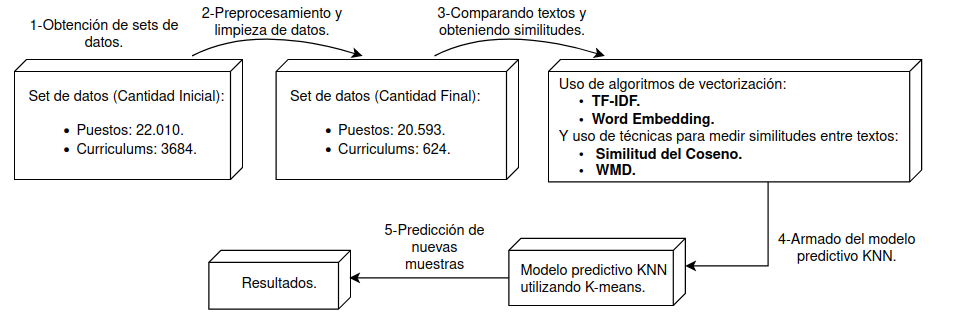
\includegraphics[width=1\textwidth]{images/flow-core.png} 	%Incluyendo imagen Flow Core.
  \caption{Pipeline Flow del Core del Sistema}  
  \label{fig:FlowCoreSystem}
\end{figure}

\subsubsection{Obtención de sets de datos.}
En primer lugar debemos definir qué es un set o conjunto de datos.
Un set o conjunto de datos es una tabla de una base de datos o, matemáticamente, una matriz estadística de datos. Cada columna de la tabla representa una variable del set de datos; y cada fila representa a un miembro determinado del mismo.

Para este Proyecto utilizamos dos grandes sets de datos que se obtuvieron mediante la recolección de distintos archivos alojados en la Web, los cuales estan descriptos a continuación.

\paragraph{Curriculum Vitae.}
Los set de datos de Curriculum Vitae de Candidatos se obtuvieron de las siguientes fuentes:

\begin{enumerate}
\item 228 Curriculums en formato docx y posteriormente convertidos a pdf, obtenidos del sitio Kaggle (https://www.kaggle.com/palaksood97/resume-dataset). Estos pdfs son Candidatos de la India con experiencia en el rubro de IT.
\item 2484 Curriculums en formato CSV, obtenidos del sitio Kagle (https://www.kaggle.com/snehaanbhawal/resume-dataset). Este CSV cuenta con CVs obtenidos del sitio web de postulación de trabajos 'livecareer.com'.
\item 962 Curriculumns en formato CSV, obtenidos del sitio Kaggle (https://www.kaggle.com/gauravduttakiit/resume-dataset). Este CSV cuenta con CVs repartidos en distintas categorías de IT.
\item 10 Curriculums en formato PDF, los cuales los cuales fueron obtenidos como ejemplos mediante una recolección propia de distintos sitios web. 
\end{enumerate}

\paragraph{Descripciones Puestos Laborales.}

Los set de datos de descripciones de puestos laborales se obtuvieron de las siguientes fuentes:

\begin{enumerate}
\item 22.000 descripciones en formato CSV; obtenido del sitio Kaggle (https://www.kaggle.com/PromptCloudHQ/us-technology-jobs-on-dicecom). El CSV cuenta con descripciones de puestos obtenidos del sitio web de USA de postulación de trabajos del rubro de IT 'Dice.com'.
\item 10 descripciones en formato CSV; obtenidas como ejemplos mediante una recolección propia del sitio Indeed (https://www.indeed.com/q-USA-jobs.html) para puestos de trabajo de IT.
\end{enumerate}
 

\subsubsection{Preprocesamiento y limpieza de datos.}
Previamente a utilizar las técnicas para medir distancias y obtener similitudes entre textos (WMD y Cosine Similarity) y los algoritmos de aprendizaje (KNN y K-Means) necesitamos que los datos que comparemos e introduzcamos en los algoritmos estén lo más limpios posible; ya que de lo contrario las mismos podrían clasificar o predecir de forma errónea. Este análisis previo sobre los datos debe ser minucioso ya que puede haber valores incoherentes o absurdos.

El procedimiento para la Limpieza de los Curriculum Vitae y las descripciones de los puestos laborales fue el siguiente:

\begin{enumerate}
\item Convertimos todo a minúscula.
\item Eliminamos datos no relevantes para nuestros análisis (mails y páginas web).
\item Eliminamos signos de puntuación y caracterés especiales (incluyendo números).
\item Eliminamos stop words.
\item Eliminamos common words no relevantes para nuestros análisis.
\item Aplicamos Lematización y Tokenización.
\item Eliminamos repetidos.
\item Obtenemos y usamos bi-gramas.
\end{enumerate}

Luego de aplicar preprocesamiento y limpieza de datos nos quedarán los siguientes tamaños de nuestros datasets:
\begin{itemize}
\item 624 CVs de Candidatos (en formato pdf y csv).
\item 20593 Descripciones de Puestos de IT (en formato csv).
\end{itemize}

\subsubsection{Cantidad final del set de datos y su uso en las distintas etapas.}

El total de CVs de Candidatos (624) y Descripciones de Puestos de IT (20593) que mencionamos previamente, serán utilizados para el entrenamiento y obtención de vectores mediante TF-IDF (para el futuro cálculo de Cosine Similarity) y para el entrenamiento de Word2Vec y obtención de los Word Embeddings (para el futuro cálculo de WMD).

Por otro lado, para calcular Cosine Similarity y WMD, para utilizarlos en K-means y para entrenar a nuestro algoritmo KNN, utilizaremos únicamente una porción de nuestros datasets:

1-Para el cálculo de Cosine Similarity y WMD:
\begin{itemize}
\item 301 CVs de Candidatos.
\item 201 Descripciones de Puestos de IT.
\end{itemize}
Nota: No obstante, al realizar los cálculos de distancias compararemos cada CV con cada Job Description, obteniendo un dataframe total de 3131 filas con sus respectivo valores de WMD y Cosine Sim.

2-Para el uso de K-means y entrenamiento con KNN (eliminamos un CV y una Descripción de Puesto IT que los utilizamos en '3-'):
\begin{itemize}
\item 300 CVs de Candidatos.
\item 200 Descripciones de Puestos de IT.
\end{itemize}        
Nota: como se comentó previamente, nos quedarán 3000 filas / puntos para usar en K-means y entrenar KNN; llegando a representar estos 3000 puntos en un plano de 2 dimensiones.

3-Para la clasificación de nuevas muestras prediciendo con KNN:
\begin{itemize}
\item 1 CV de Candidatos.
\item 1 Descripción de Puesto de IT.
\end{itemize}
Nota: como se comentó previamente, nos quedarán 131 filas para clasificar.

¿Por qué utilizamos solo una porción de nuestros datasets?: Esto es debido a los drawbacks de WMD y KNN.
\begin{itemize}
\item WMD: posee una alta complejidad en el cálculo de la distancia, teniendo un tiempo de ejecución muy elevado. Como ejemplo, al correrlo localmente, el cálculo de WMD para 3131 filas tardó 7 horas; frente a los 3 segundos que tardó el cálculo de Cosine Similarity para la misma cantidad de filas.
\item KNN: KNN es una gran opción para datasets pequeños con pocas variables de entrada; pero tiene problemas cuando la cantidad de entradas es muy grande. Cada variable de entrada puede considerarse una dimensión de un espacio de entrada p-dimensional. En grandes dimensiones, los puntos que pueden ser similares pueden tener distancias muy grandes. Además, cada vez que se va a hacer una predicción con KNN, busca al vecino más cercano en el conjunto de entrenamiento completo. Por esto, se debe utilizar un dataset pequeño para que el clasificador KNN completa su ejecución rápidamente.
\end{itemize}
En conclusión, al utilizar solo una porción de nuestros datasets para obtener los distintos cálculos de distancias y entrenar KNN, el cálculo de WMD se podrá realizar en un tiempo finito, y nuestro clasificador KNN funcionará rápida y eficientemente al realizar predicciones.

\subsection{Comparando textos y obteniendo similitudes.}
\colorbox{red}{FALTA}

Previamente a utilizar Cosine Similarity y WDM para (-----completar-----) se debe emplear algún algoritmo de vectorización que permita representar las palabras de nuestros textos a un espacio vectorial. De esta forma Cosine Similarity y WMD podrán interpretarlos de la mejor manera. 
Como mencionamos previamente, como algoritmos de vectorización se utilizarán TF-IDF y Word Embeddings.


\subsection{Armado del modelo predictivo KNN.}
\colorbox{red}{FALTA}

\subsection{Predicción de nuevas muestras y resultados obtenidos.}
\colorbox{red}{FALTA}

\subsection{Integración al Sistema Web.}
\colorbox{red}{FALTA}

Como mencionamos, el Sistema se integrará a un framework para tener una UI accesible.
El framework Web utilizado será..... COMPLETAR.
E


; y se tendrán 2 tipos de usuario: 
*  Reclutador. 
*  Candidatos.
Los Reclutadores cargarán en el Sistema los puestos de trabajo que tengan disponibles.
Y los Candidatos …..COMPLETAR.


\subsubsection{Base de datos.}
\colorbox{red}{FALTA}

\subsubsection{Secciones del sistema}

Para registrarse o loguearse al sistema, se implementará la interfaz provista en la figura \ref{fig:Vista_Registro}.

\begin{figure}[H]    %[H] es para que se ubique justo debajo del texto anterior. 
  \centering
  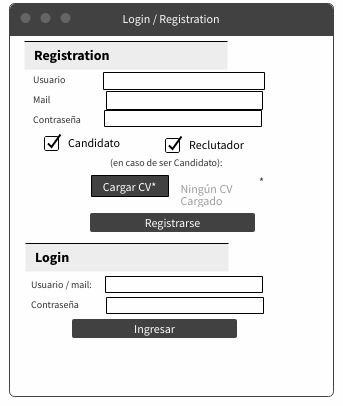
\includegraphics[width=1\textwidth]{images/Vista_Registro.png}
  \caption{Logueo y Registración.}  
  \label{fig:Vista_Registro}
\end{figure}

\colorbox{red}{ES UN BOCETO, FALTA PONER LA IMAGEN REAL}

El Candidato tendrá acceso al menú indicado en la figura \ref{fig:Vista_Candidato}. 

\begin{figure}[H]    %[H] es para que se ubique justo debajo del texto anterior. 
  \centering
  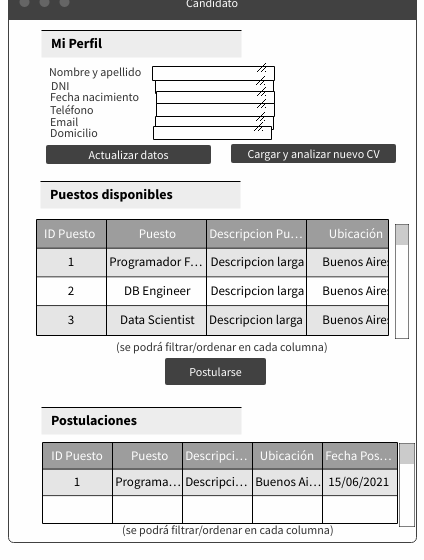
\includegraphics[width=1\textwidth]{images/Vista_Candidato.png}
  \caption{Vista del Candidato.}  
  \label{fig:Vista_Candidato}
\end{figure}

\colorbox{red}{ES UN BOCETO, FALTA PONER LA IMAGEN REAL}

Por su parte, el Reclutador tendrá acceso al menú indicado en la figura \ref{fig:Vista_Reclutador}. 

\begin{figure}[H]    %[H] es para que se ubique justo debajo del texto anterior. 
  \centering
  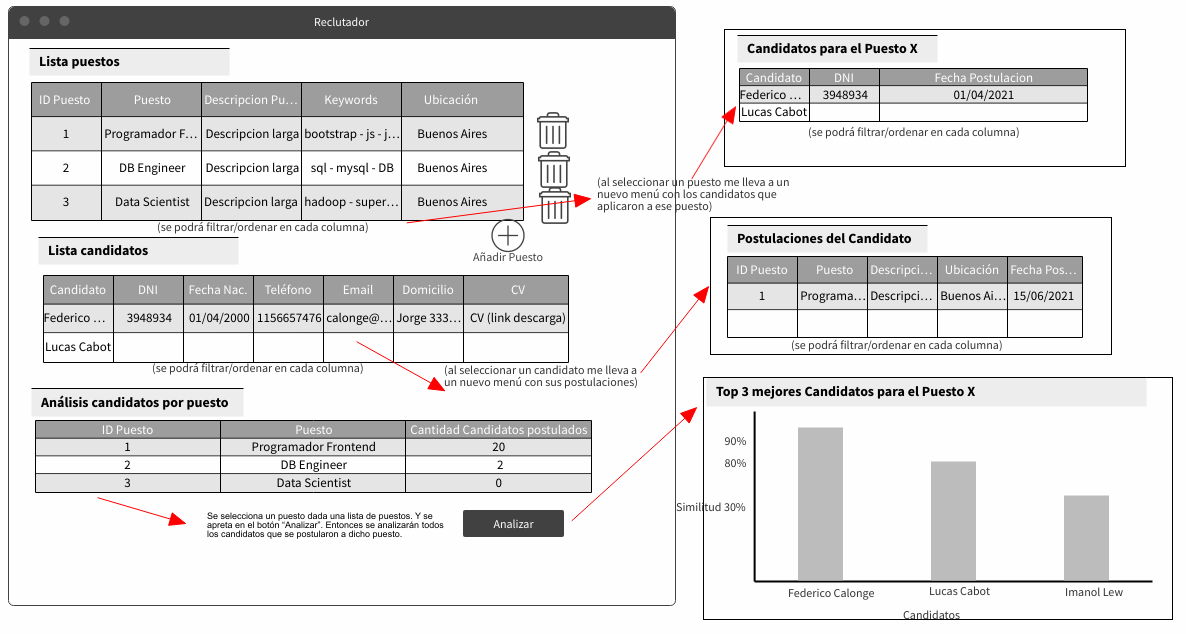
\includegraphics[width=1\textwidth]{images/Vista_Reclutador.png}
  \caption{Vista del Reclutador.}  
  \label{fig:Vista_Reclutador}
\end{figure}

\colorbox{red}{ES UN BOCETO, FALTA PONER LA IMAGEN REAL}

\subsubsection{Manejo de los datos.}
\colorbox{red}{FALTA}

\paragraph{Modelado.}
\colorbox{red}{FALTA}

\paragraph{Filtrado.}
\colorbox{red}{FALTA}

\paragraph{Visualización.}
\colorbox{red}{FALTA}

\subsection{Pipeline Flow final del Sistema.}
\colorbox{red}{FALTA}

Una vez que el reclutador dentro de la sección observada en la figura \ref{fig:Vista_Reclutador} haga click en "Analizar", el sistema reflejará el pipeline indicado en la figura \ref{fig:Pipeline_Final} para obtener como resultado final un TOP de los 3 mejores candidatos para el puesto solicitado (considerando que dichos candidatos hayan aplicado a dicho puesto). 

\begin{figure}[H]    %[H] es para que se ubique justo debajo del texto anterior. 
  \centering
  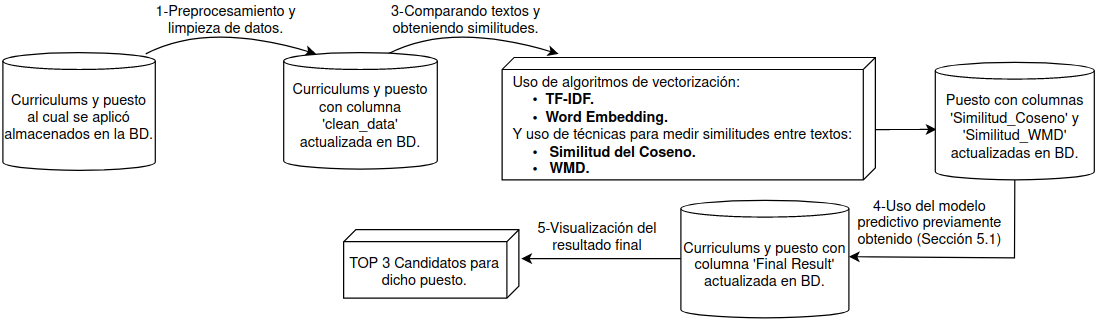
\includegraphics[width=1\textwidth]{images/Pipeline_Final.png}
  \caption{Pipeline Flow final del Sistema.}  
  \label{fig:Pipeline_Final}
\end{figure}

\subsection{Conclusiones.}
\colorbox{red}{FALTA}

\subsection{Caso de Uso.}
\colorbox{red}{FALTA}

\subsection{Limitaciones del sistema.}
\colorbox{red}{FALTA}
 
\section{Próximos pasos.}  
\colorbox{red}{FALTA - acá poner mejoras}

\section{Glosario.}
\colorbox{red}{FALTA}

\section{Anexos.}
\colorbox{red}{FALTA}
\cleardoublepage


\begin{thebibliography}{9}
\bibitem{ejemplo}
Autor1, \& Autor2. (Año, mes). \textit{TITULO}. Año y conferencia (pp. 0971-0974). IEEE.

\end{thebibliography}



\end{document}


%Para poner pie de paginas --> \footnote{Un conjunto de datos, conocido también como dataset, es una colección de datos habitualmente tabulada.})

%Para poner en Las citas del anexo --> información\cite{iot}. 

